\section{Heterogeneidad Verdadera}
\label{sec:heterogeneidad-verdadera}

Para ampliar las capacidades de Heterogenius extendimos el concepto de heterogeneidad para lograr tener demostraciones verdaderamente heterogeneas en lugar de demostraciones heterogéneas pero con secuentes homogéneos. 

La diferencia principal radica en que, con la nueva implementaci'on, los secuentes pueden soportar f'ormulas de diferentes lenguajes. As'i un secuente puede ser de tipo homogéneo o heterogéneo. En el primer caso todas las f'ormulas del secuente usan el mismo lenguaje; en el segundo las f'ormulas son de lenguajes distintos.

La ventaja de los secuentes heterogéneos es que se pueden combinar f'ormulas (lemmas, axiomas) provenientes de distintas especificaciones escritas en lenguajes diferentes. De esta forma nos podemos abstraer del lenguaje en el que están escritas y concentrarnos en el an'alisis.

La principal limitaci'on de los secuentes heterogéneos es que las herramientas (calculadores de secuentes, buscadores de contraejemplos, demostradores autom'aticos) trabajan con secuentes escritos en un solo lenguaje, o sea secuentes homogéneos. Debido a esto se proveen nuevas operaciones para el manejo de f'ormulas dentro de un secuente:

\subsection{Operaciones para el manejo de f'ormulas}

Cada una de las siguientes operaciones puede cambiar o no la heterogeneidad de un secuente.  Dependiendo de los lenguajes de las f'ormulas del resultado, el secuente puede pasar a ser heterogéneo, homogéneo o mantener su tipo.

\subsubsection{Proyecci'on}

'Esta operaci'on  permite seleccionar un subconjunto de las f'ormulas que se quiere proyectar sobre el secuente actual y el nuevo secuente se forma a partir de las f'ormulas seleccionadas.
Dado un secuente: $$ \alpha_1,\ldots,\alpha_n \vdash \alpha_{n+1},\ldots,\alpha_m $$
%% \begin{prooftree}
%% \AxiomC{$\alpha_1$,$\ldots$,$\alpha_n$}
%% \UnaryInfC{$\alpha_{n+1}$,$\ldots$,$\alpha_m$}
%% \end{prooftree}
y un subconjunto $\mathcal{C} \subseteq \{1 \ldots m\}$, el secuente resultante de la proyecci'on es el siguiente:
%% \begin{prooftree}
%% \AxiomC{$\alpha_i$ con $i=1 \ldots n$ y $i \in \mathcal{C}$}
%% \UnaryInfC{$\alpha_j$ con $j=n+1 \ldots m$ y $j \in \mathcal{C}$}
%% \end{prooftree}
$$\{\alpha_i \} \vdash \{\alpha_j\} \mbox{ con }i\in [1,n]\cap\mathcal{C} \mbox{ y } j\in [n+1, m]\cap\mathcal{C}$$
%\vspace{1em}

Si se aplica una operaci'on de proyecci'on a un secuente homog'eneo el resultado siempre ser'a homog'eneo, pero si se empieza con un secuente heterogeneo el resultado puede ser un secuente homog'eneo, si se proyectan f'ormulas de un mismo lenguaje o un secuente heterog'eneo si la proyecci'on incluye f'ormulas de lenguajes diferentes.

A modo de ejemplo, en la Fig.~\ref{seq selection} se muestra el cuadro de di'alogo mediante el cual el usuario puede marcar las f'ormulas que se quiere proyectar en el nuevo secuente.

\begin{figure}[tb]
	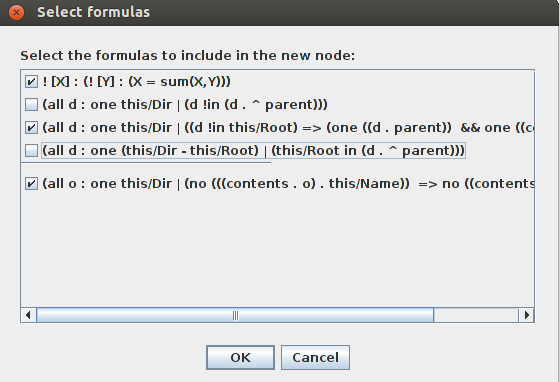
\includegraphics[width=200px]{img/select.png}
	\centering
	\caption{Cuadro de di'alogo de proyecci'on de f'ormulas.}
        \label{seq selection}
\end{figure}

\subsubsection{Introducci'on de antecedentes desde una fuente externa}

'Esta operaci'on permite cargar f'ormulas desde un archivo de especificaci'on, ya sea escrito en el lenguaje \textit{Alloy} o en \textit{TPTP-FOF}, e introducirlas como nuevas hip'otesis en el secuente actual.

Dado un secuente:
$$ \alpha_1,\ldots,\alpha_n \vdash \alpha_{n+1},\ldots,\alpha_m $$
y un conjunto de f'ormulas nuevas $\{\beta_1 \ldots \beta_k\}$. El nuevo secuente es:
$$ \alpha_1,\ldots,\alpha_n,\beta_1,\ldots, \beta_k \vdash \alpha_{n+1},\ldots,\alpha_m $$

'Esta operaci'on puede puede conservar o cambiar tanto la homogeneidad como la heterogeneidad del secuente inicial.

\begin{figure}
\centering
\parbox{5cm}{
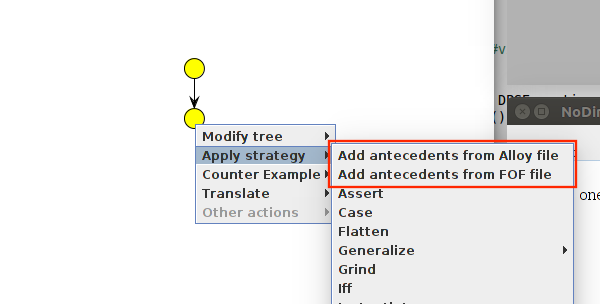
\includegraphics[width=5cm]{img/add_antecedents_1.png}	
\caption{Menu contextual para seleccionar la fuente de las f'ormulas a introducir.}}
\qquad
\begin{minipage}{5cm}
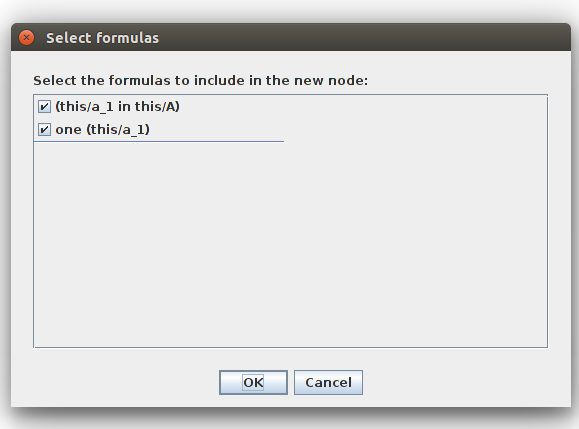
\includegraphics[width=5cm]{img/add_antecedents_2.png}
\caption{Dialogo para seleccionar las f'ormulas.}
\end{minipage}	
\end{figure}


\subsubsection{Traducci'on}

Se extendi'o el concepto de traducciones $\rho$ para que se puedan traducir f'ormulas por separado, en lugar de traducir un secuente completo como en la versi'on anterior.
El secuente resultante contendr'a las f'ormulas del secuente analizado en el lenguaje seleccionado.

Dado un secuente $$ S: \alpha_1,\ldots,\alpha_n \vdash \alpha_{n+1},\ldots,\alpha_m $$
y una función  $\mathcal{T}:Formula\rightarrow Lenguaje$ que indica el lenguaje seleccionado para cada f'ormula del secuente $S$, el secuente resultante es:
$$ S': \beta_1,\ldots,\beta_n \vdash \beta_{n+1},\ldots,\beta_m $$
donde $\beta_{i} = \rho_{\mathcal{T}(\alpha_i)}(\alpha_i)$ y $\rho_l$ es la funci'on de traducci'on al lenguaje $l$.

En la Figura \ref{GUI form translation} se puede ver un cuadro de di'alogo donde el usuario puede seleccionar, para cada f'ormula, el lenguaje al que se quiere traducir.

\begin{figure}[tb]
	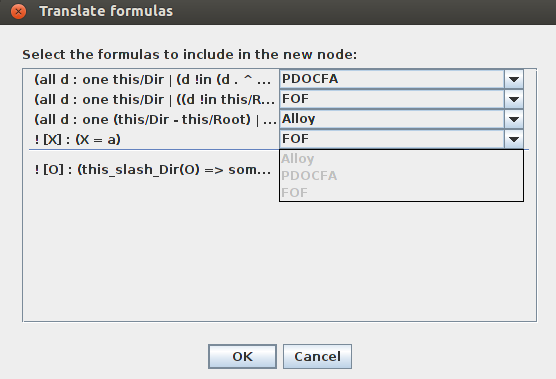
\includegraphics[width=200px]{img/translate.png}
	\centering
	\caption{Cuadro de di'alogo para la traducci'on de f'ormulas en un secuente.} \label{GUI form translation}
\end{figure}


%á
